\documentclass{article}
\usepackage[left=3cm,right=3cm,top=2cm,bottom=2cm]{geometry} 
\usepackage{makeidx}         % allows index generation
\usepackage[pdftex]{graphicx,color}          % standard LaTeX graphics tool
\DeclareGraphicsRule{.pdftex}{pdf}{.pdftex}{}
                             % when including figure files
\usepackage{multicol}        % used for the two-column index
\usepackage[bottom]{footmisc}% places footnotes at page bottom

\usepackage{amssymb}
\usepackage{amsmath}
\usepackage{pifont}
\usepackage{bm}
\usepackage{cancel}
\usepackage{multirow}
\usepackage{amsmath}
\usepackage{epstopdf}
\usepackage[caption=false,font=footnotesize]{subfig}


\DeclareMathOperator*{\argmin}{arg\,min}

\DeclareGraphicsExtensions{.eps, .pdf, .png, .jpg}
\graphicspath{{./images/},{./}}

\newcommand{\red}[1]{{\color{red}#1}}
\renewcommand{\vec}[1]{\bm{#1}}
\newcommand{\mat}[1]{\bm{#1}}
\newcommand{\cframe}[1]{$\langle #1 \rangle$}
\newcommand{\prescript}[2]{\phantom{}^{#1}_{#2}}

\newcommand\frontmatter{%
    \cleardoublepage
%%  \@mainmatterfalse
  \pagenumbering{roman}}
\newcommand\mainmatter{%
    \cleardoublepage
%%  \@mainmattertrue
  \pagenumbering{arabic}}
%%%%%%%%%%%%%%%%%%%%%%%%%%%%%%%%%%%%%%%%%%%%%%%%%%%%%%%%%%%%%%%%%%%%%

\begin{document}
\frontmatter
\onecolumn 
\vskip 1cm
%\pagestyle{empty}
\begin{center}
\huge \textsc{Cooperative Robotics}\\
\vskip 1cm

\skip 0.5cm

\vskip 5cm

\normalsize
Authors: Astha Gupta\\
EMAILs: astha736@gmail.com \\
Date: \\
\end{center}
\clearpage
\mainmatter
\section*{General Concepts}

Following the notations from the main notes. The configuration of the system is the vector of its DOF parameters.

\begin{equation}
c \triangleq\left[\begin{array}{l}{q} \\ {\eta}\end{array}\right]
\end{equation}

where q is the configuration of the arm. 

\begin{equation}
\boldsymbol{q} \triangleq\left[\begin{array}{c}{q_{1}} \\ {\vdots} \\ {q_{n}}\end{array}\right]
\end{equation}

Configuration of the vehicle base is given as below:

\begin{equation}
\eta \triangleq\left[\begin{array}{l}{\eta_{1}} \\ {\eta_{2}}\end{array}\right] \in \mathbb{R}^{6}
\end{equation}

\begin{equation}
\eta_{1} \triangleq\left[\begin{array}{l}{x} \\ {y} \\ {z}\end{array}\right], \eta_{2} \triangleq\left[\begin{array}{l}{\phi} \\ {\theta} \\ {\psi}\end{array}\right]
\end{equation}

\begin{equation}
\dot{y}=\left[\begin{array}{l}{\dot{q}} \\ {\nu}\end{array}\right] \quad \nu=\left[\begin{array}{l}{\nu_{1}} \\ {\nu_{2}}\end{array}\right] \quad \begin{array}{l}{\nu_{1}=^{v} v} \\ {\nu_{2}=^{v} w}\end{array}
\end{equation}

The relationship between the derivative of Euler(RPY) angles and vehicle-base's angular velocity is given the below equation.   
\begin{equation}
\left[\begin{array}{c}{\dot{\phi}} \\ {\dot{\theta}} \\ {\dot{\psi}}\end{array}\right]=\left[\begin{array}{ccc}{1} & {\tan (\theta) \sin (\phi)} & {\tan (\theta) \cos (\phi)} \\ {0} & {\cos (\phi)} & {-\sin (\phi)} \\ {0} & {\frac{\sin (\phi)}{\cos (\theta)}} & {\frac{\cos (\phi)}{\cos (\theta)}}\end{array}\right] \boldsymbol{\nu}_{2}
\end{equation}

\begin{itemize}
	\item Thus in the code the Jacobian expected is between $^{w}\dot{x}$, in the world frame ${w}$ and $^{b}\dot{y}$, in the body frame ${b}$. 
	
	\begin{equation}
	^{w} \dot{\boldsymbol{x}}=\boldsymbol{J}  ^{b}\dot{\boldsymbol{y}}
	\end{equation}
	
	where the components of velocity of the vehicle frame are expressed in the body frame. 
	
	\item The basic functionality listed below has already been implemented.
	\begin{itemize}
		\item "ha": Horizontal Altitude
		\item "mu": Manipulability
		\item "t": Tool Position Control
	\end{itemize}
\end{itemize}


\clearpage


\section{Exercise 1: Implement a “Safe Waypoint Navigation” Action.}

\subsection{Adding a vehicle position control objective}
Initialize the vehicle far away from the seafloor. An example position could be
\begin{displaymath}
\begin{bmatrix} 10.5 & 35.5 & -36 & 0 & 0 & \pi/2\end{bmatrix}^\top
\end{displaymath} 
Give a target position that is also sufficiently away from the seafloor, e.g.,
\begin{displaymath}
\begin{bmatrix} 10.5 & 37.5 & -38 & 0 & 0 & 0 \end{bmatrix}^\top
\end{displaymath}

Goal: Implement a vehicle position control task, and test that the vehicle reaches the required position and orientation.


\subsubsection{Q1: Report the hierarchy of task used and their priorities. What is the Jacobian relationship for the Vehicle Position control task? How was the task reference computed?}
\begin{itemize}
	\item Hierarchy of Task used and their priorities \\
	 The tasks used for the first questions are listed below. The priority of the task is the same as the enumeration, where the number increase as the priority decreases.
	\begin{enumerate}
		\item "ha": Horizontal Altitude
		\item "posc": Vehicle Position Control 
		\item "mu": Manipulability
		\item "t": Tool Position Control	
	\end{enumerate}
	For this task Horizontal Altitude is given the maximum priority, to avoid situations where the robot is upside down. Since in this project the code for the desired behaviour is being incrementally built, the position-control was the only task added at this step to the base code. 
	
	Postion Control does not require Manipulability and Tool Position-Control, but they were kept to understand their effect on the overall task. Thus they could be switched off if the robot is only required to perform Position-Control. 
	
	\item Jacobian Relationship for Vehicle Position Control 
	
	
	\begin{equation}
	\left[\begin{array}{c}{^{w}\dot{v}_{3 \times 1}} \\ ^{w}{\omega}_{3 \times 1}\end{array}\right]=\left[\begin{array}{ccc}{\mathbf{0}_{3 \times 7}} & {^{w}\boldsymbol{R}_{v}}& {\mathbf{0}_{3 \times 3}} \\ {\mathbf{0}_{3 \times 7}} & {\mathbf{0}_{3 \times 3}} & { ^{w}\boldsymbol{R}_{v}}\end{array}\right]\left[\begin{array}{c}{\dot{q}_{7 \times 1}} \\ ^{b}{v}_{3 \times 1} \\ ^{b}{\omega}_{3 \times 1}\end{array}\right]
	\end{equation}
	
	
	\item Task Reference Computation \\
	The reference velocity $\dot{x}_{ref}$ is computed using the Cartesian Error between the goal pose(vehicle-base) and current vehicle-base pose in the world frame, using the "CartError" function, and scaling it with appropriate factor $\lambda$. For this task $\lambda = 0.2 $
	
	\begin{equation}
	^{w}\dot{\boldsymbol{x}}_{ref}=\lambda \left[\begin{array}{c}{\delta{r} } \\ {\delta{\theta}}\end{array}\right]^{w}
	\end{equation}
	
\end{itemize}

\subsubsection{Q2: What is the behaviour if the Horizontal Attitude is enabled or not? Try changing the initial or target orientation in terms of roll and pitch angles. Discuss the behaviour.}

To understand the difference between behaviour, we conducted  4 runs of the simulation using different parameters as stated below. 

\begin{itemize}
	\item Default priority (dp): $ \left[ "ha", "posc", "mu", "t" \right]$ 
	\item Horizontal priority off (haOff):  $ \left[ "posc", "mu", "t" \right]$ 
	\item Target default (tdef): $ \left[10.5, 37.5, -38, 0, 0, 0 \right]$ 
	\item Target new (tnew): $ \left[10.5, 37.5, -38, degtorad(45), degtorad(45), 0 \right]$  
\end{itemize}

\begin{figure}[!h]
\subfloat[(dp,tdef)\label{fig:1a}]{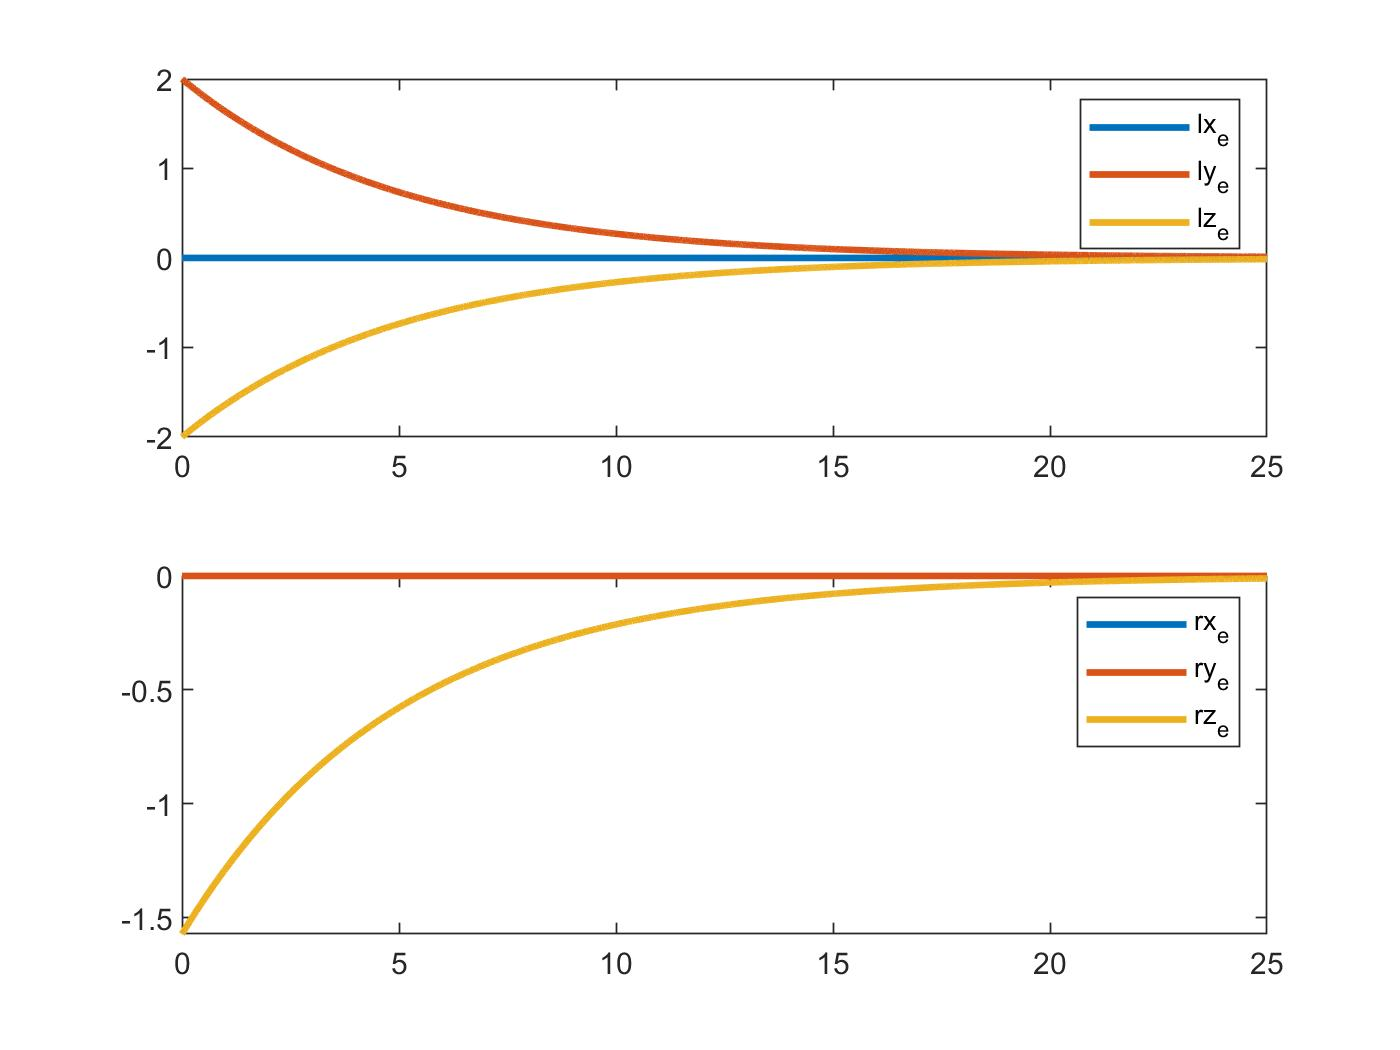
\includegraphics[width=.6\linewidth]{Task1/priority_posc/init_rpy/5}}\hfill
\subfloat[(dp,tnew)\label{fig:1a}]{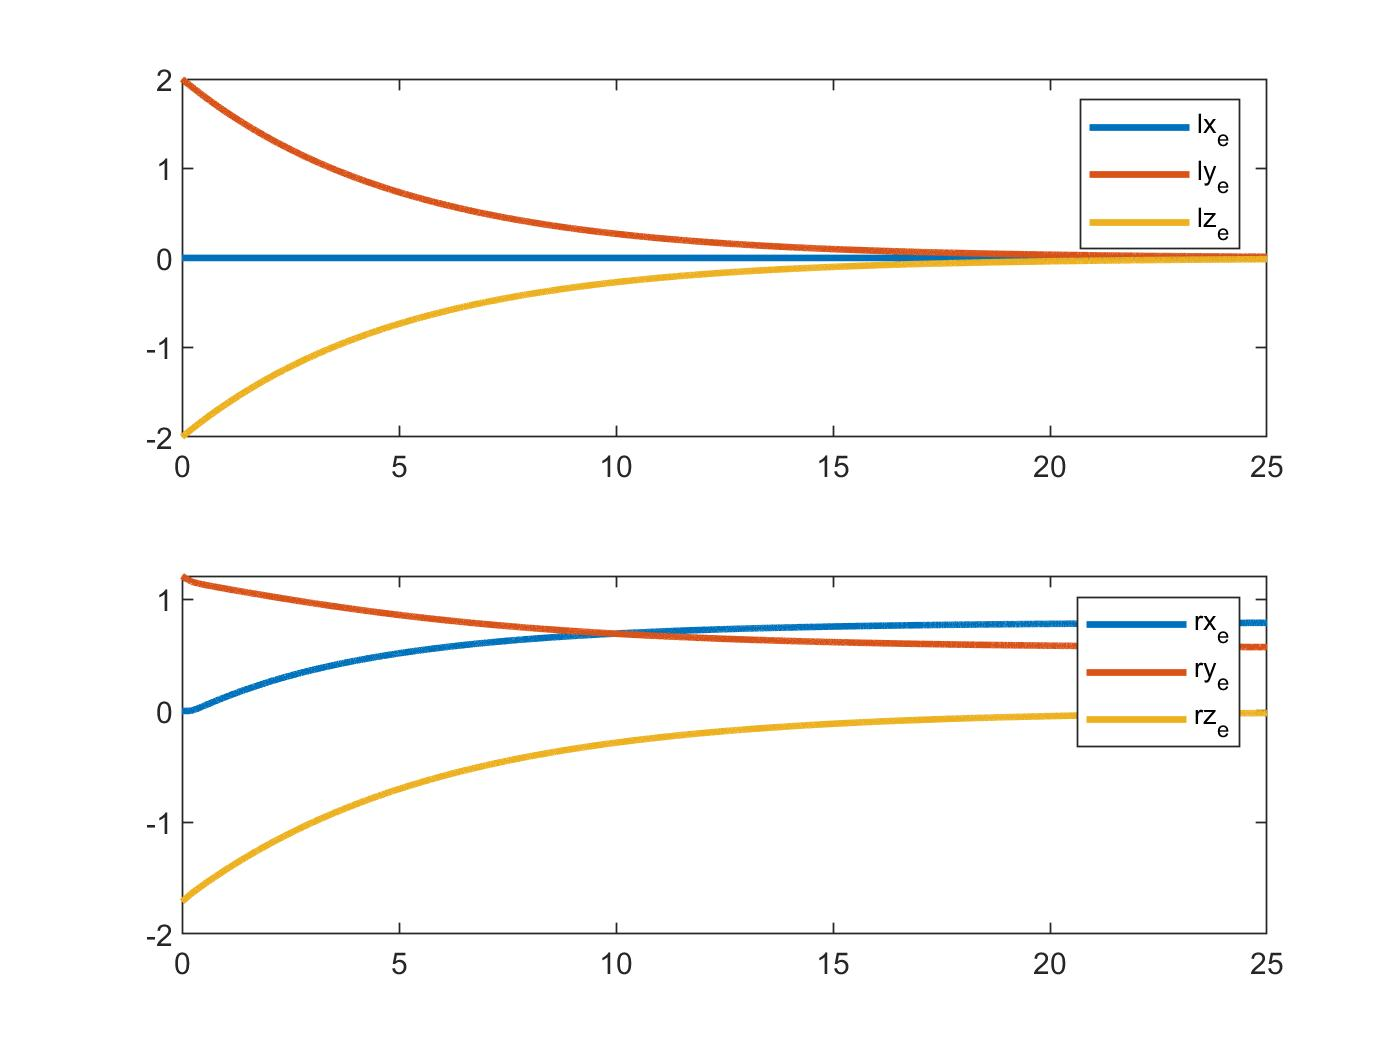
\includegraphics[width=.6\linewidth]{Task1/priority_posc/rpy_45_45_0/5}}\hfill
\subfloat[(haOff,tdef)\label{fig:1a}]{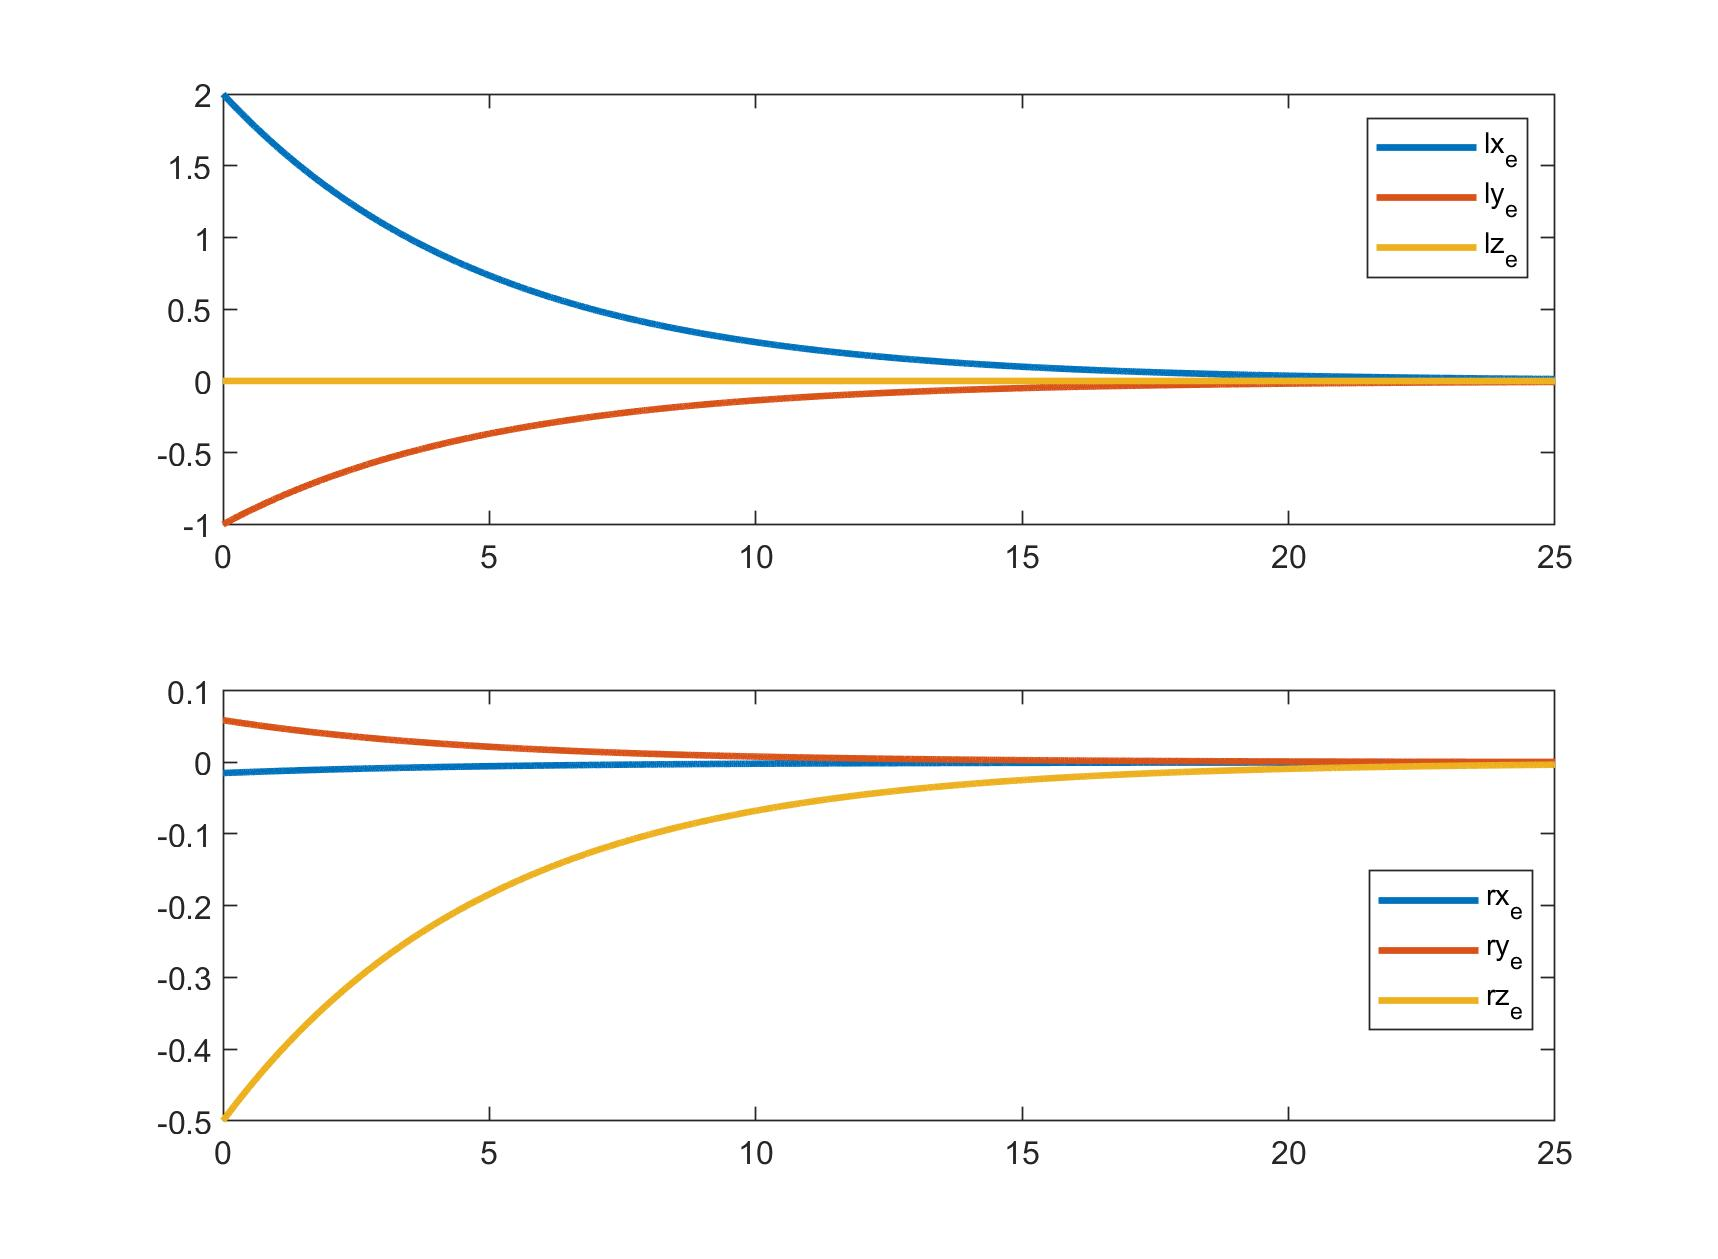
\includegraphics[width=.6\linewidth]{Task1/priority_ha_off/init_rpy/5}}\hfill
\subfloat[(haOff,tnew)\label{fig:1a}]{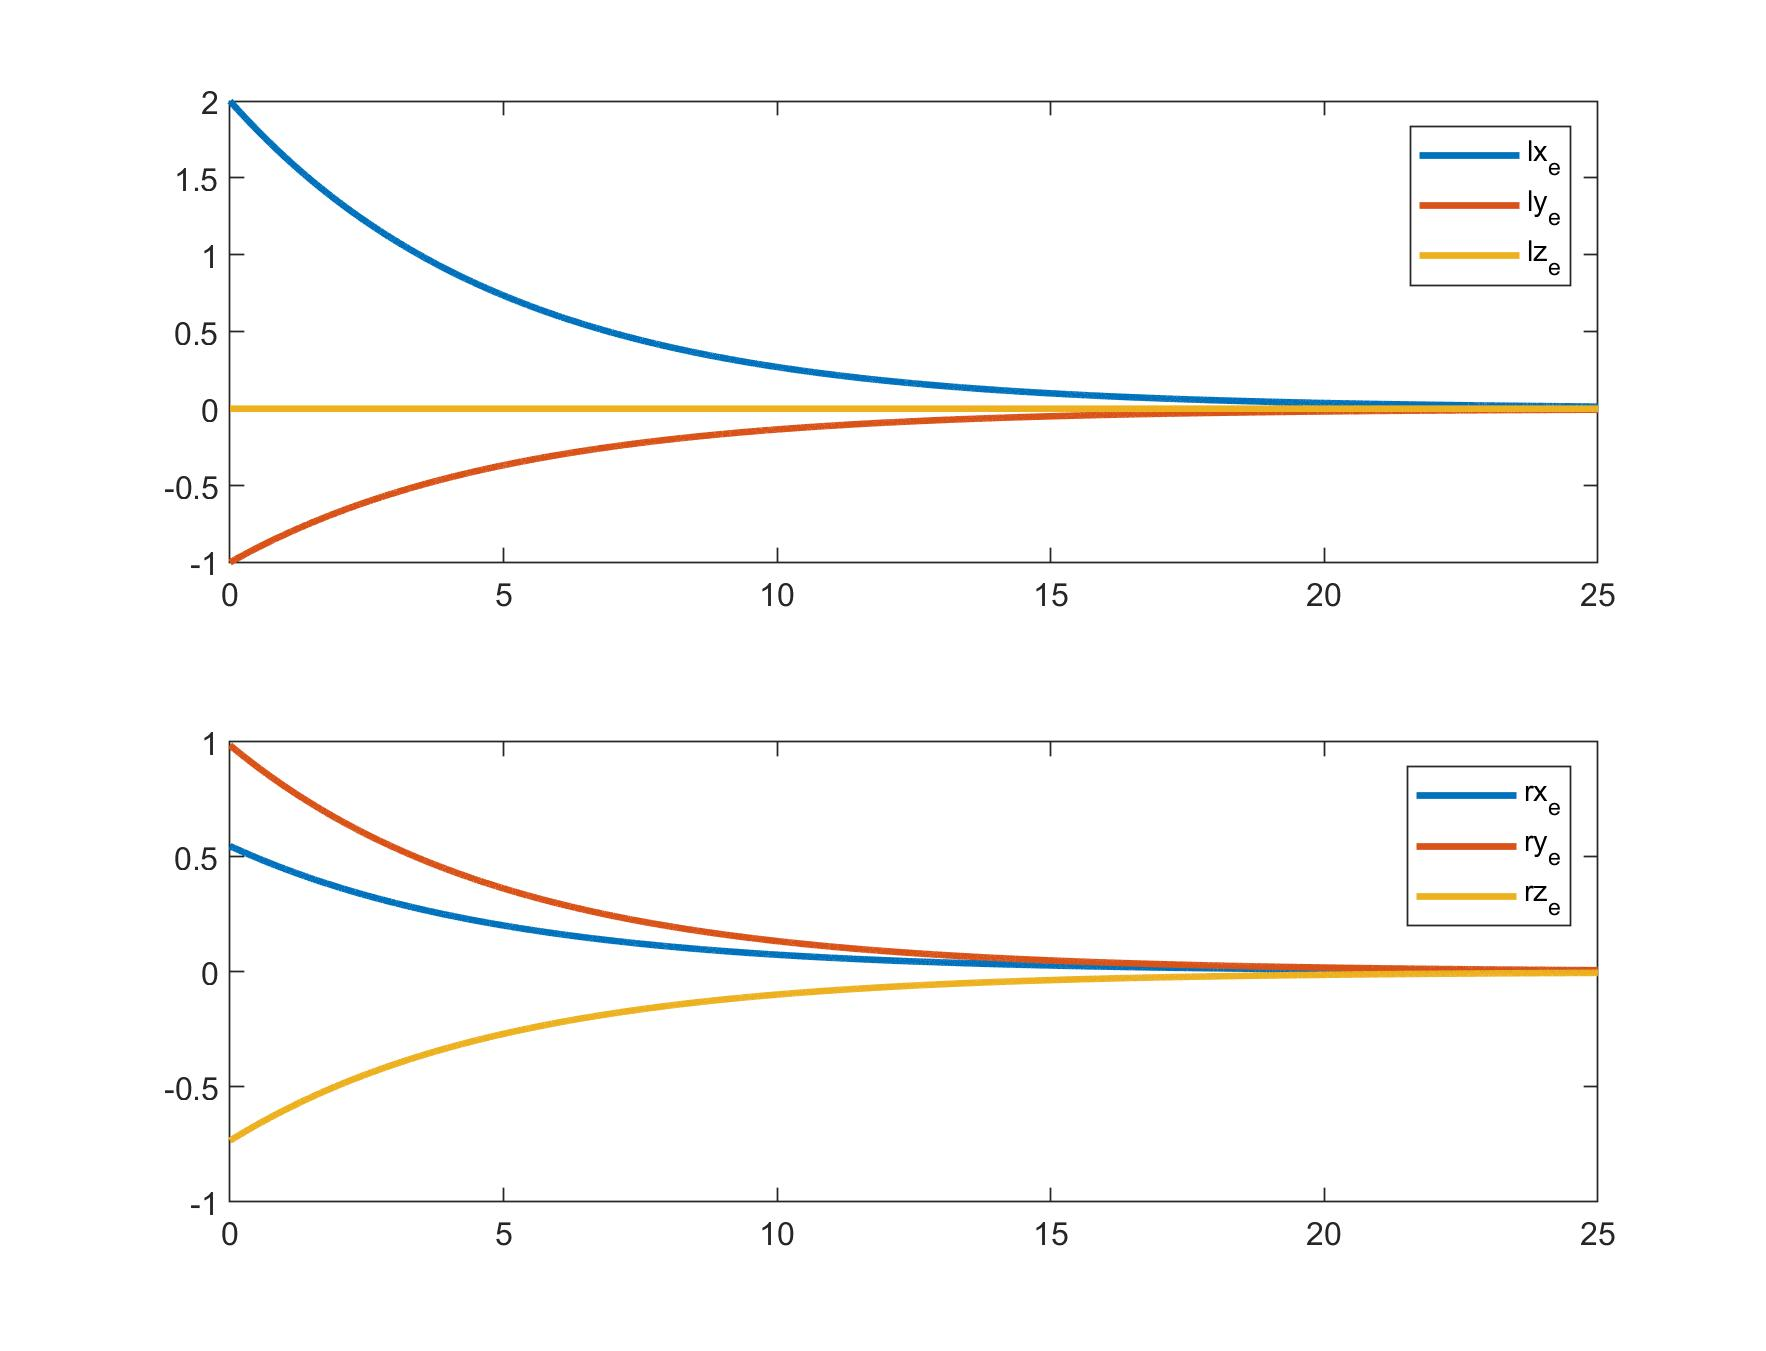
\includegraphics[width=.6\linewidth]{Task1/priority_ha_off/rpy_45_45_0/5}}\hfill
\end{figure}


\begin{figure}[!h]
	\subfloat[(dp,tdef)\label{fig:1a}]{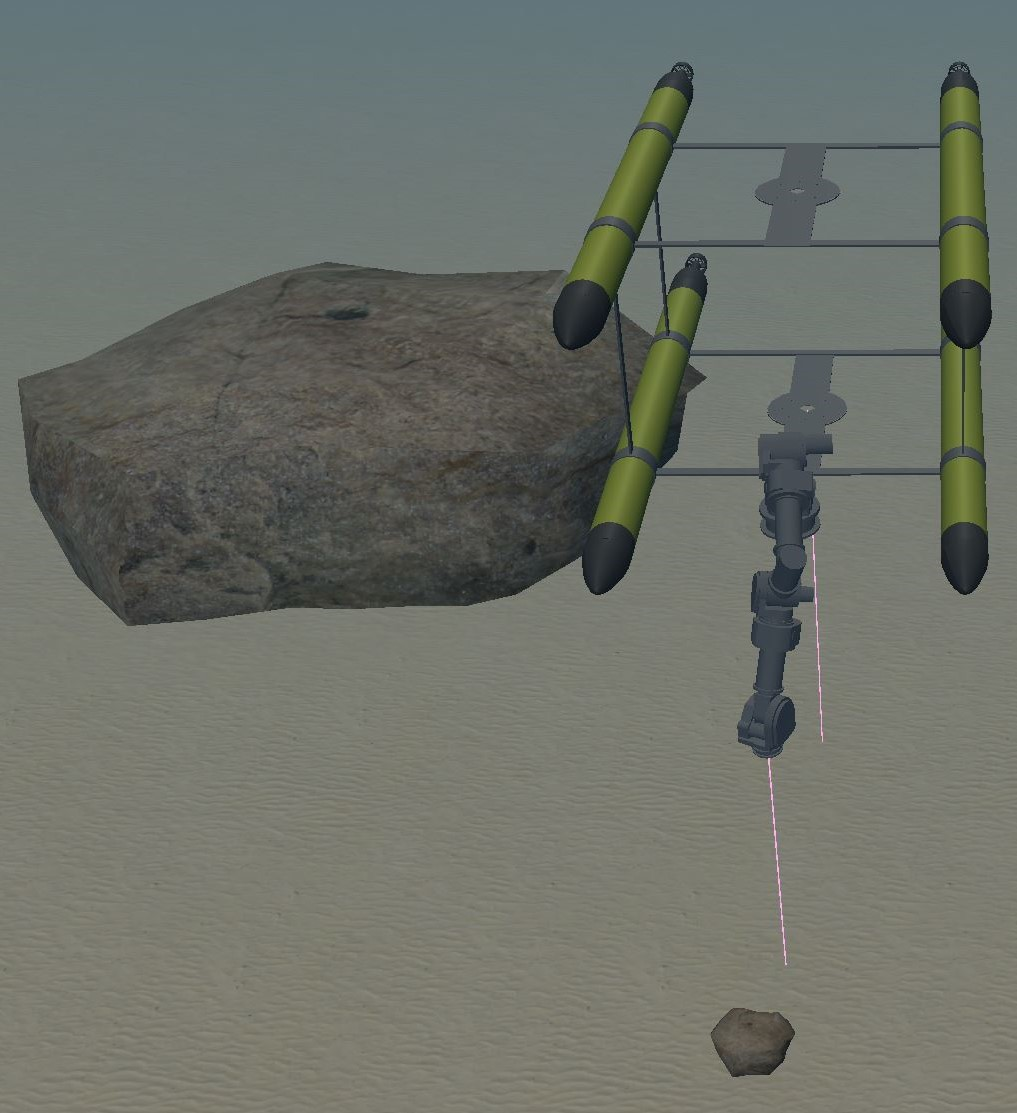
\includegraphics[width=.165\linewidth]{Task1/priority_posc/init_rpy/task1_posc_c}}\hfill
	\subfloat[(dp,tnew)\label{fig:1a}]{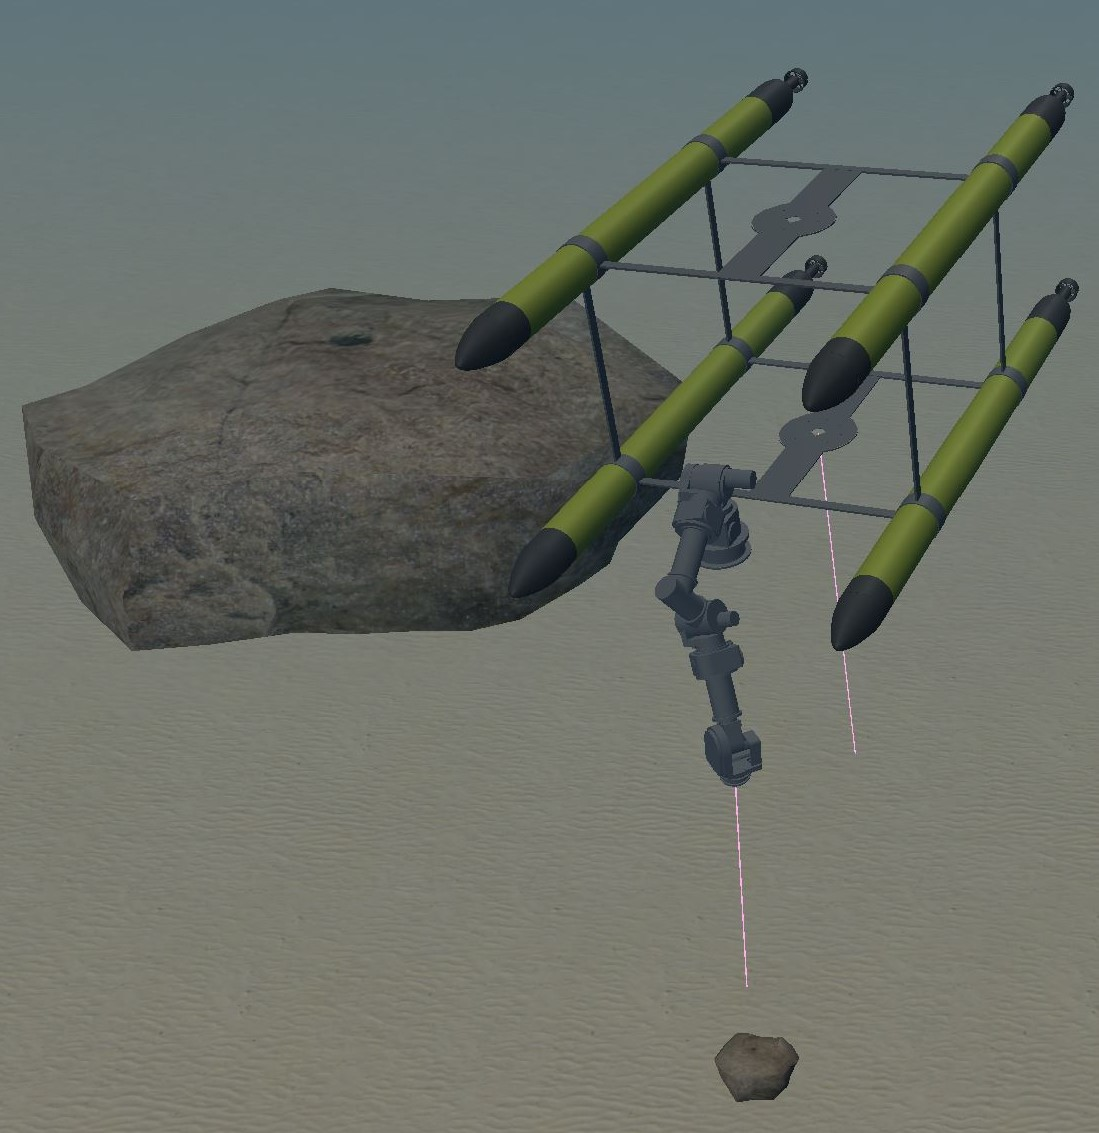
\includegraphics[width=.190\linewidth]{Task1/priority_posc/rpy_45_45_0/task1_posc_c}}\hfill
	\subfloat[(haOff,tdef)\label{fig:1a}]{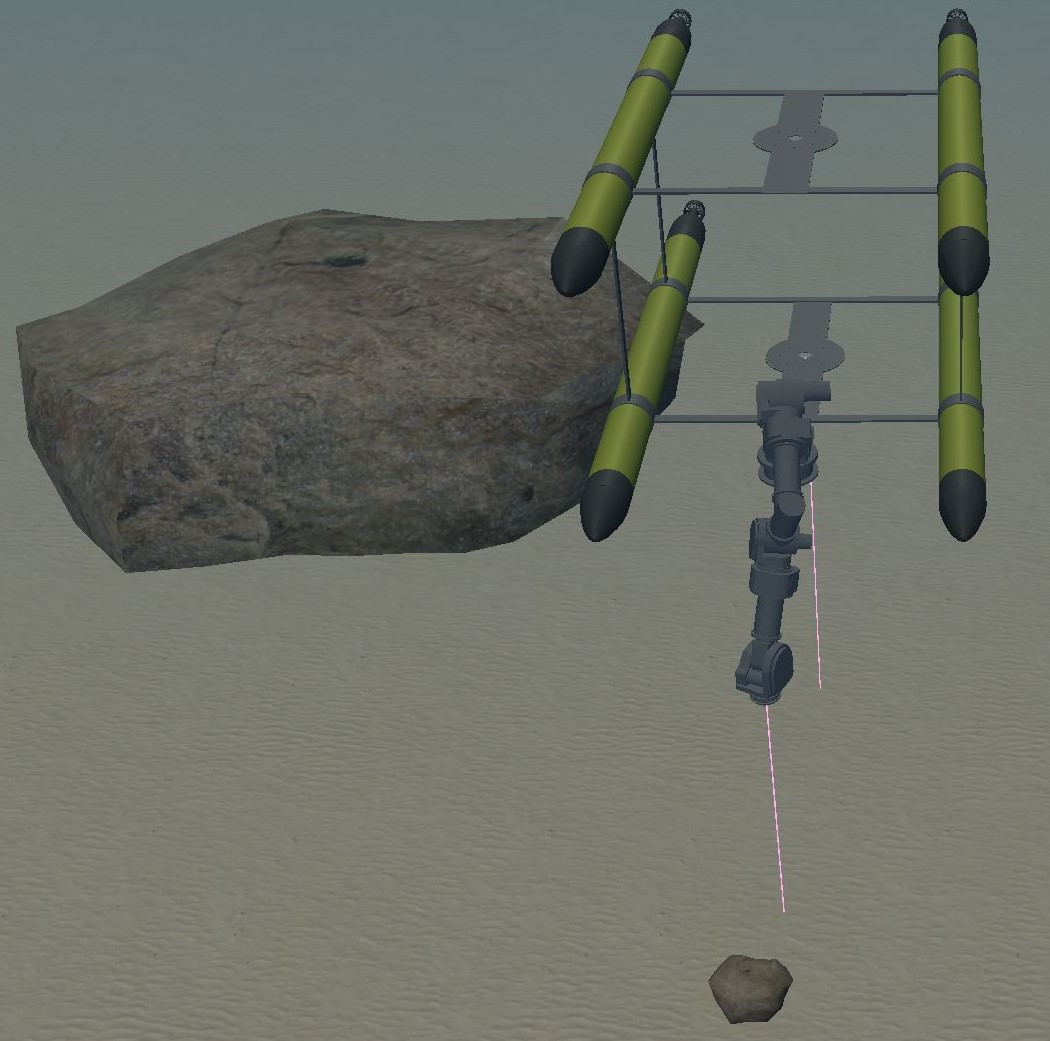
\includegraphics[width=.2\linewidth]{Task1/priority_ha_off/init_rpy/task1_c}}\hfill
	\subfloat[(haOff,tnew)\label{fig:1a}]{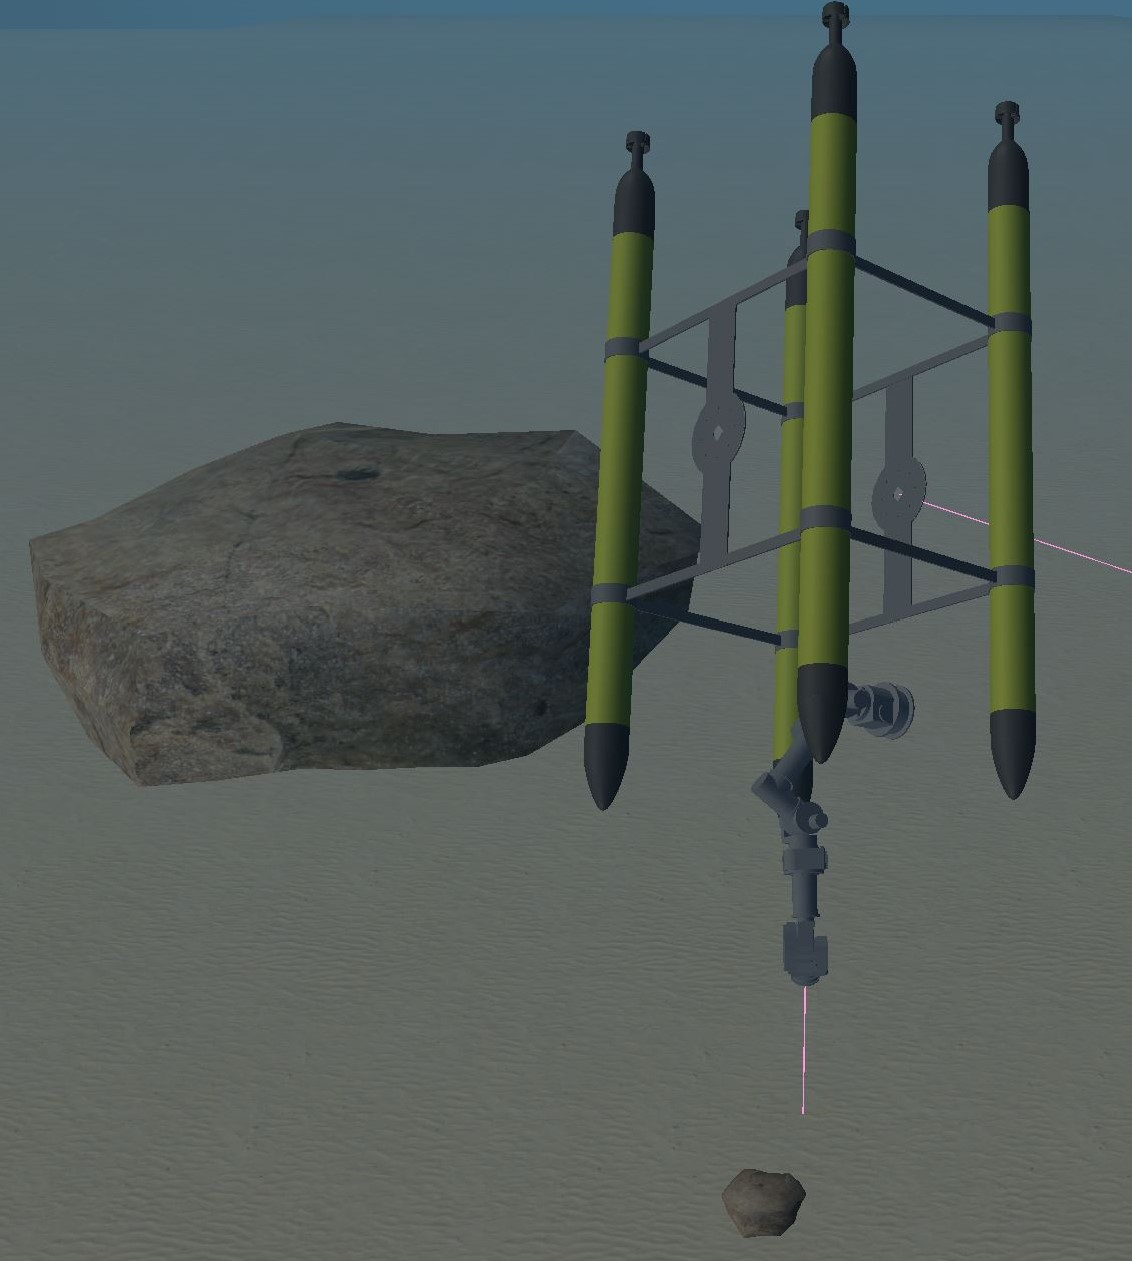
\includegraphics[width=.150\linewidth]{Task1/priority_ha_off/rpy_45_45_0/task1_c}}\\
\end{figure}

As we see that in the first case where the default priority is used the errors do not converge for the tnew position, as the position-control and horizontal altitude have conflicting goals. Since the "ha" has higher priority, the target is not achieved for the second case. 

Were as the (c) and (d) part "ha" is off, thus the errors for vehicle-base converge to zero, but the robot is flipped in part (d). 

\subsubsection{Q3: Swap the priorities between Horizontal Attitude and the Vehicle Position control task. Discuss the behaviour.}

Since for target position tdef there is no substantial conflict of goals between "ha" and "posc", here we are omitting the graphs and instead focusing on results for tnew. 
The switched priority is (haSwt):  $ \left[ "posc","ha", "mu", "t" \right]$ 

\begin{figure}[!h]
	\subfloat[(dp,tnew)\label{fig:1a}]{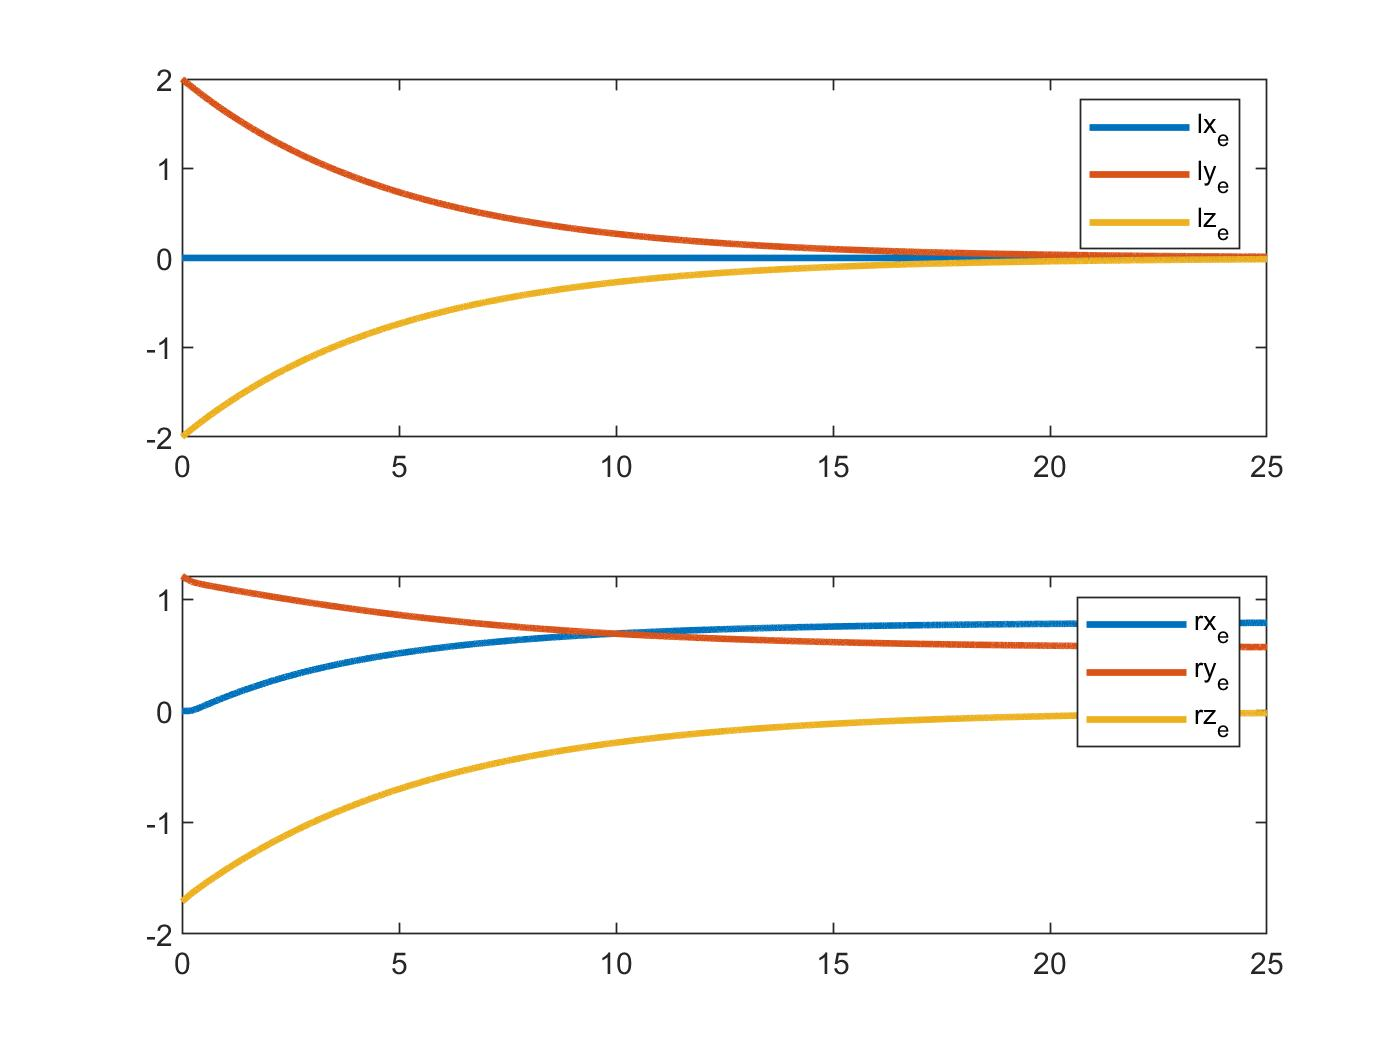
\includegraphics[width=.6\linewidth]{Task1/priority_posc/rpy_45_45_0/5}}\hfill
	\subfloat[(dp,tnew)\label{fig:1a}]{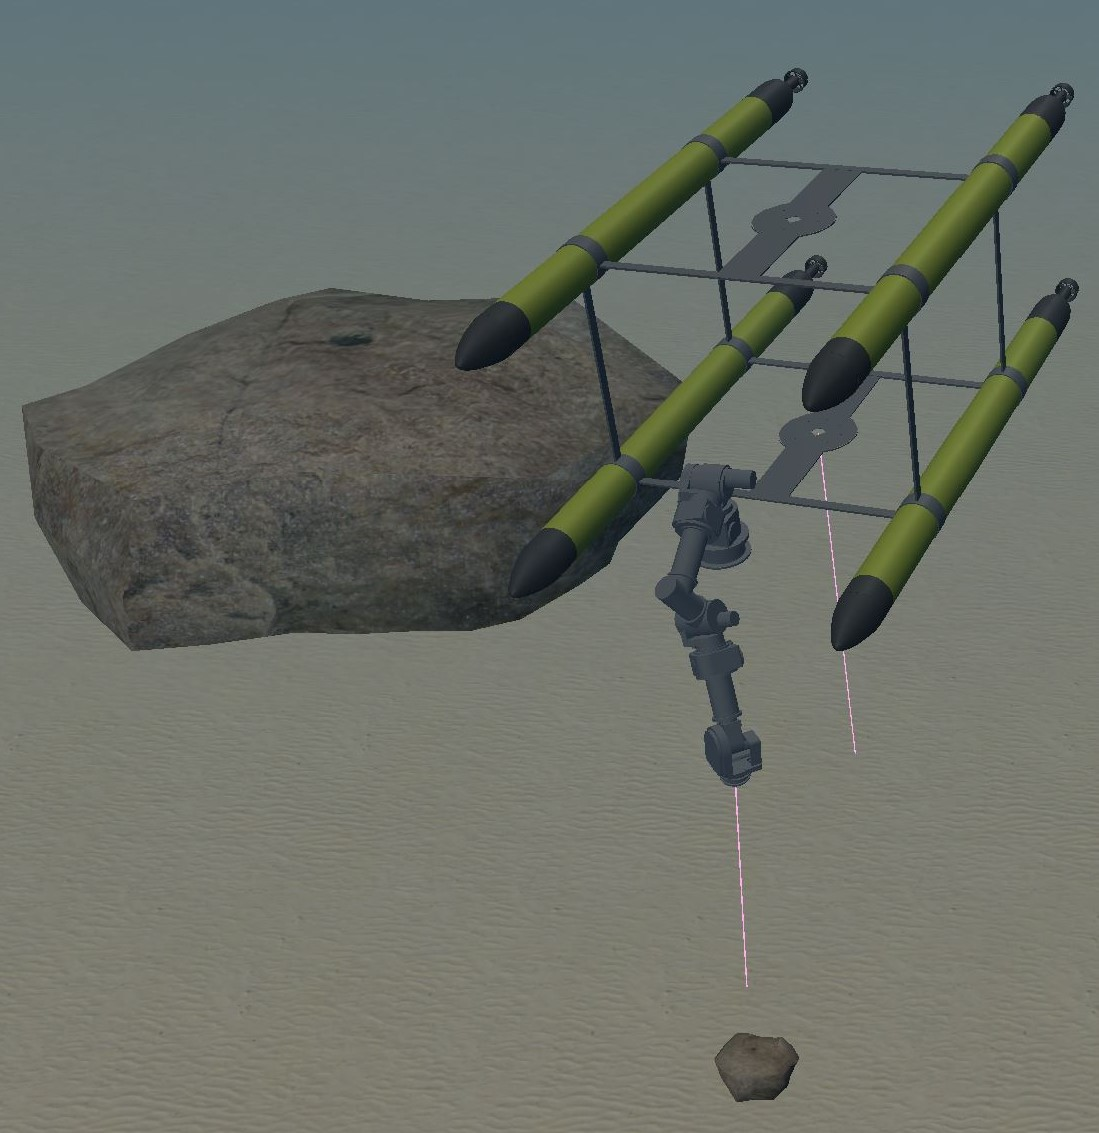
\includegraphics[width=.390\linewidth]{Task1/priority_posc/rpy_45_45_0/task1_posc_c}}\hfill
	\subfloat[(haSwt,tnew)\label{fig:1a}]{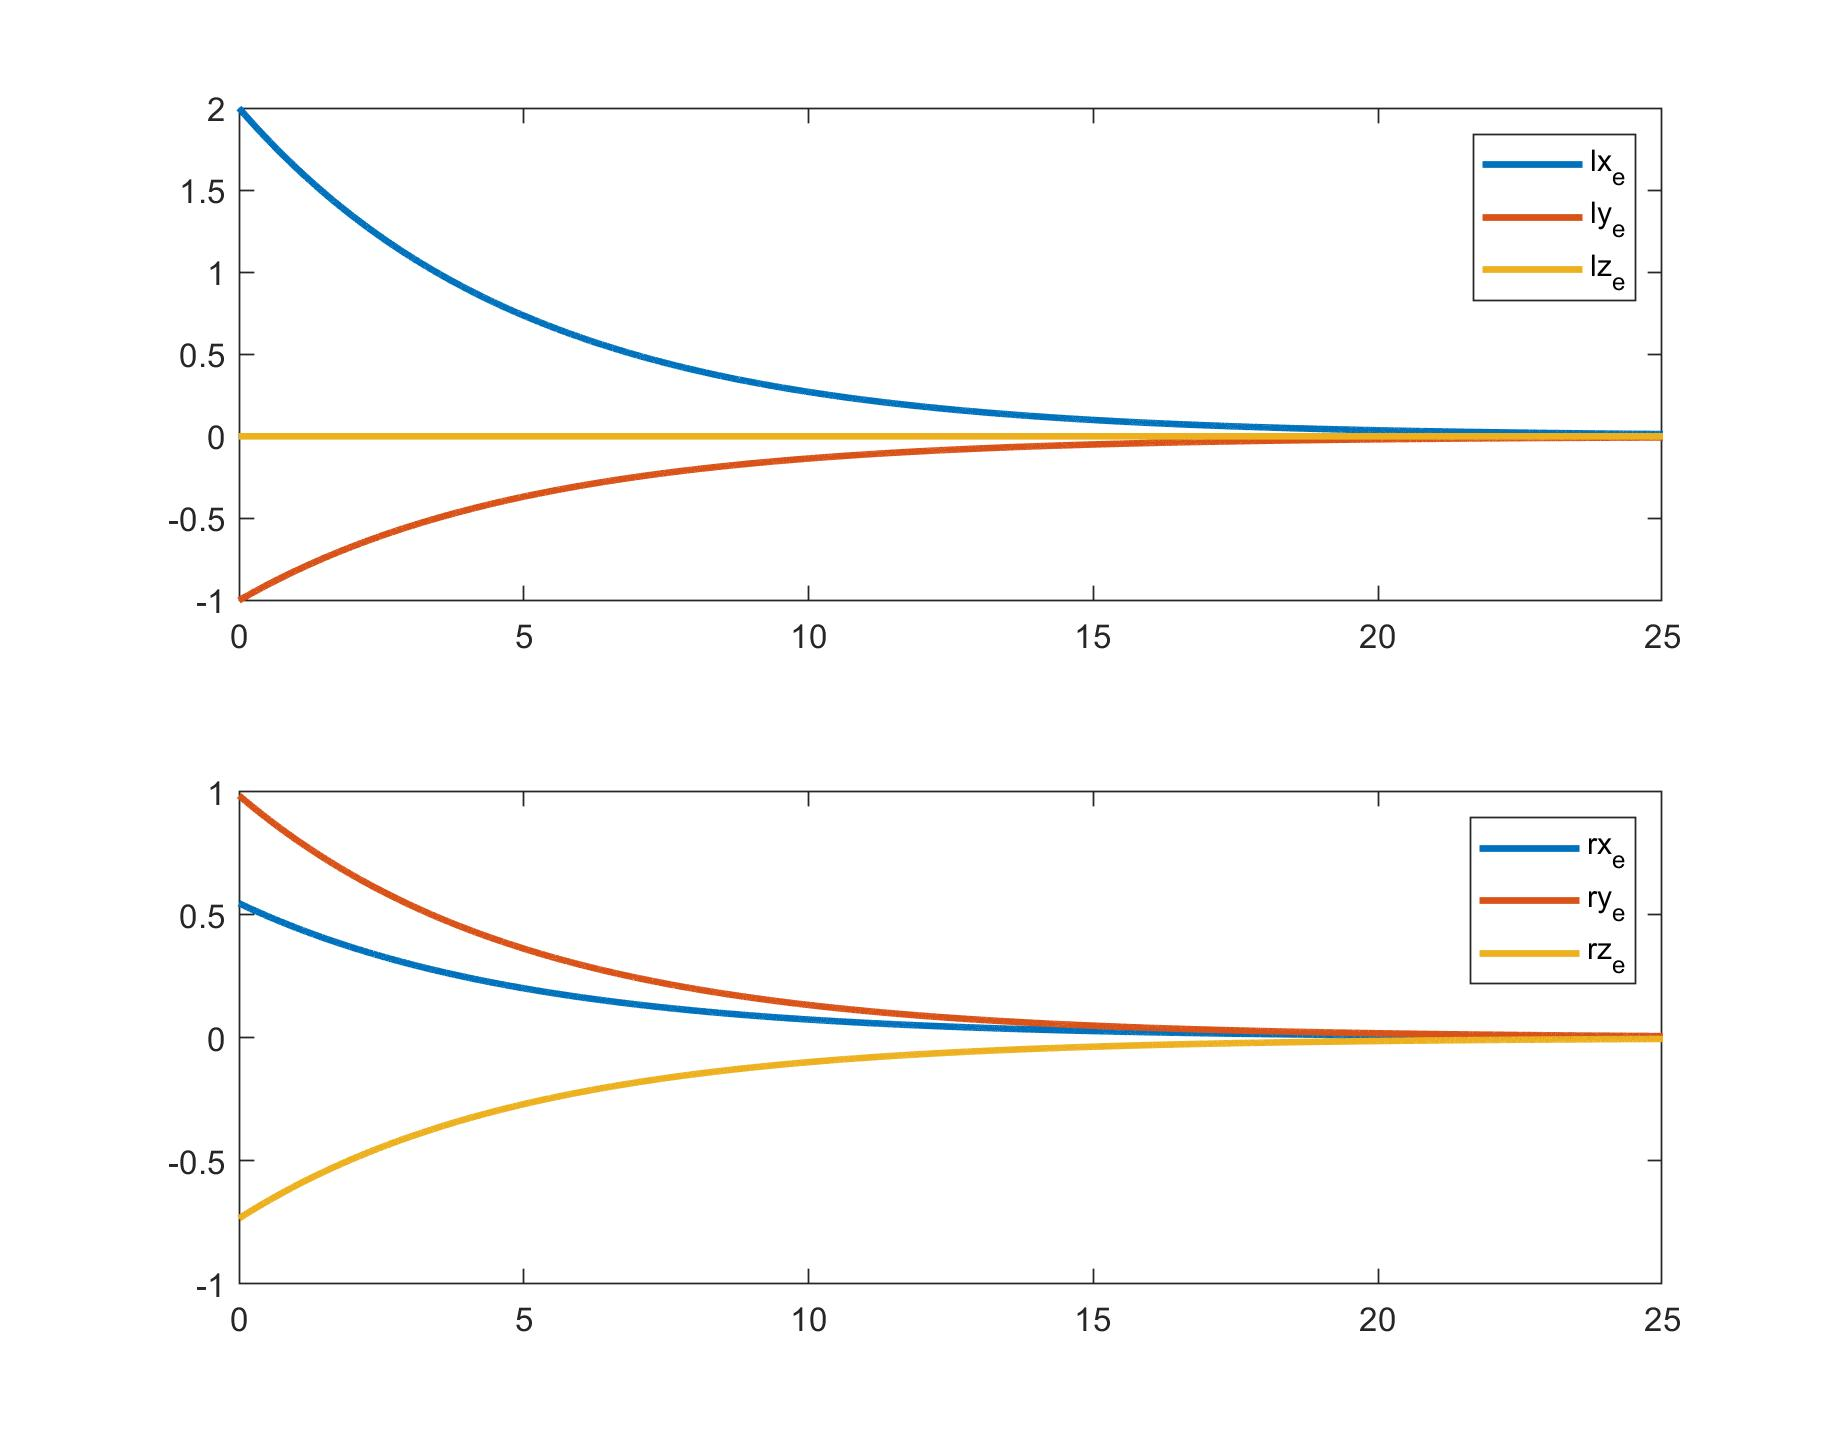
\includegraphics[width=.6\linewidth]{Task1/priority_posc_ha_switch/rpy_45_45_0/5}}\hfill
	\subfloat[(haSwt,tnew)\label{fig:1a}]{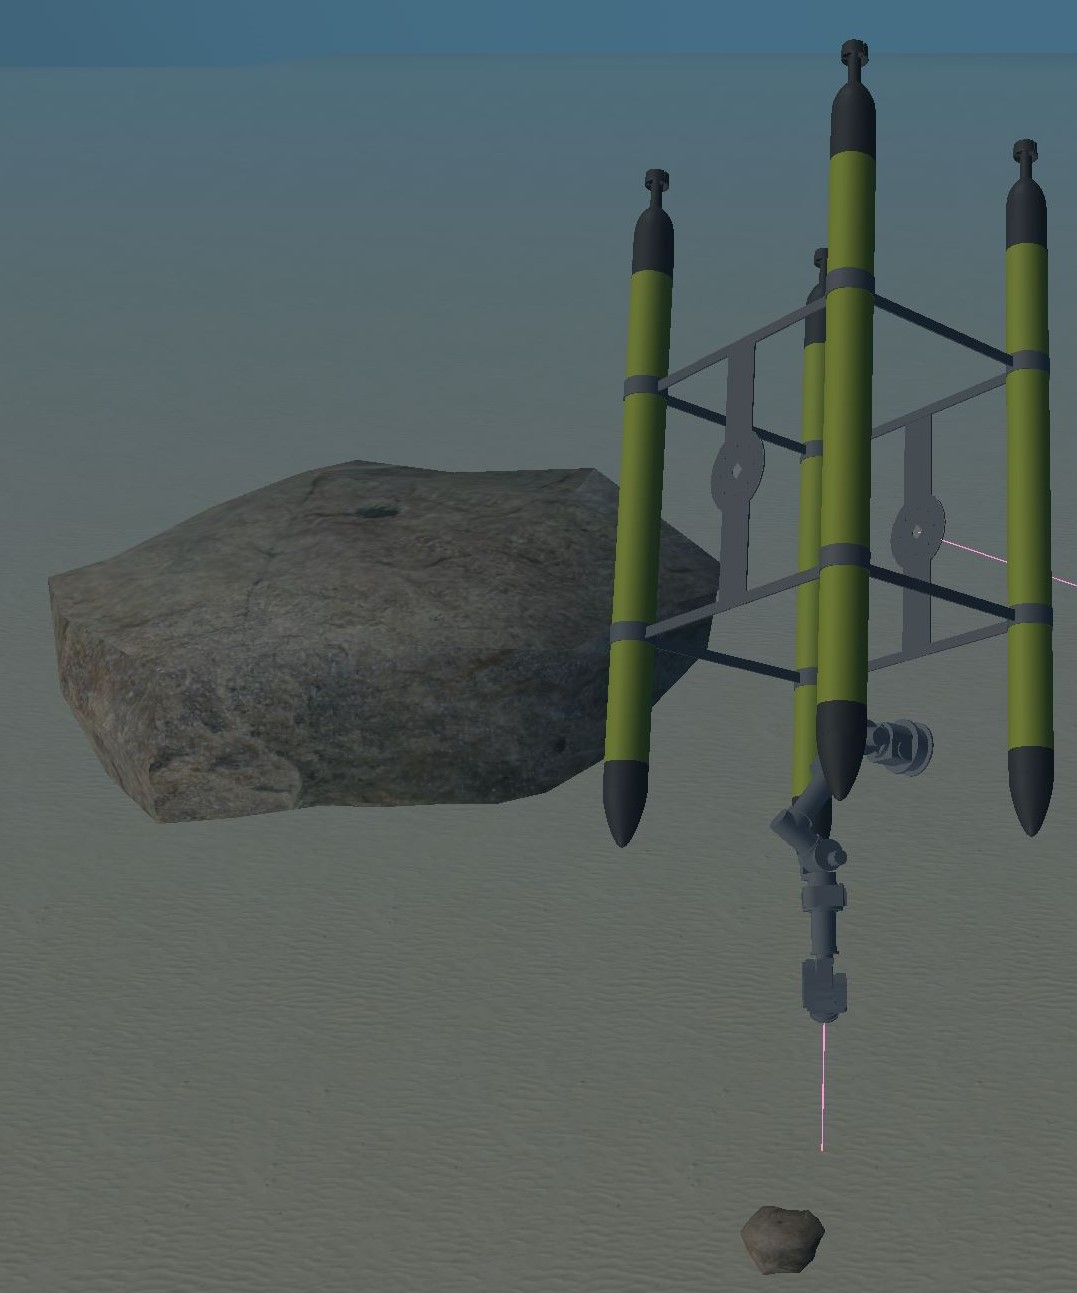
\includegraphics[width=.350\linewidth]{Task1/priority_posc_ha_switch/rpy_45_45_0/task1_posc_c}}\\
\end{figure}

As expected in the case of default priority the "ha" takes precedence and hence the vehicle is not able to achieve a zero error for "posc". Whereas in the switched proprity case the errors for position goes to zero, but the vehicle is flipped. 

\subsubsection{Q4: What is the behaviour if the Tool Position control task is active and what if it is disabled? Which of the settings should be used for a Safe Waypoint Navigation action?}

The behaviour of the robot with respect to achieving required pose is the same. The activation for, joint velocity remains 0 and there is no change in configuration of joints. Although there is no impact of Tool position control on vehicle position control in our case, it should be disabled for safe waypoint nagivation to avoid possible colision and any other unanticipated behaviour.


\subsection{Adding a safety minimum altitude control objective}
Initialize the vehicle at the position:
\begin{displaymath}
\begin{bmatrix} 48.5 & 11.5 & -33 & 0 & 0 &-\pi/2\end{bmatrix}^\top
\end{displaymath} 
Choose as target point for the vehicle position the following one:
\begin{displaymath}
\begin{bmatrix} 50 & -12.5 & -33 & 0 & 0 & -\pi/2 \end{bmatrix}^\top
\end{displaymath}

Goal: Implement a task to control the altitude from the seafloor. Check that at all times the minimum distance from the seafloor is guaranteed.


\subsubsection{Q1: Report the hierarchy of task used and their priorities. Comment how you choose the priority level for the minimum altitude.}

The hierarchy used is given below. Since the Minimum Altitude is a safety feature so that the vehicle does not crash into the sea floor, thus it has been given the highest priority. 

\begin{enumerate}
	\item "mac": Minimum Altitude Control
	\item "ha": Horizontal Altitude
	\item "posc": Vehicle Position Control 
	\item "mu": Manipulability
	\item "t": Tool Position Control	
\end{enumerate}


\subsubsection{Q2: What is the Jacobian relationship for the Minimum Altitude control task? How was the task reference computed?}

The Jacobian "Jmac" is given as below:  
\begin{equation}
\left[\begin{array}{c}{^{w}\dot{v}_{3 \times 1}} \\ ^{w}{\omega}_{3 \times 1}\end{array}\right]=\left[\begin{array}{ccc}{\mathbf{0}_{3 \times 7}} & {^{w}\boldsymbol{R}_{v}}& {\mathbf{0}_{3 \times 3}} \\ {\mathbf{0}_{3 \times 7}} & {\mathbf{0}_{3 \times 3}} & {\mathbf{0}_{3 \times 3}}\end{array}\right]\left[\begin{array}{c}{\dot{q}_{7 \times 1}} \\ ^{b}{v}_{3 \times 1} \\ ^{b}{\omega}_{3 \times 1}\end{array}\right]
\end{equation}

The reference velocity is given by 
\begin{displaymath}
\begin{bmatrix} 0 & 0 & {v}_z & 0 & 0 & 0 \end{bmatrix}^\top
\end{displaymath}

%\begin{equation}
%$^{w}\dot{\boldsymbol{v}_{z}=\lambda \left[\begin{array}{c}{ minimum threshold - sensor distance  }\end{array} \right]$
%\end{equation}

\begin{equation}
{\boldsymbol{v}}_{z}=\lambda \left[ minimum.threshold - floor.distance \right]
\end{equation}


where sensor distance is the distance from sea floor given by the sensors on the vehicle.




\subsubsection{Q3: Try imposing a minimum altitude of 1, 5, 10 m respectively. What is the behaviour?}

\subsubsection{Q4: How was the sensor distance processed?}

The distance given by the sensor of the vehicle is in the z direction of the body frame. As the body frame's z axis may not be parallel to the world frame's z axis, thus the displacement vector (with only z component) was projected to the world frame. For our calculation we used only the z component of the projected vector as it would be the actual distance between the vehicle and the sea floor. 

\clearpage

\section{Exercise 2: Implement a Basic “Landing” Action.}
\subsection{Adding an altitude control objective}
Initialize the vehicle at the position:
\begin{displaymath}
\begin{bmatrix} 10.5 & 37.5 & -38 & 0 & -0.06 & 0.5 \end{bmatrix}^\top
\end{displaymath} 

Goal: add a control task to regulate the altitude to zero.

\subsubsection{Q1: Report the hierarchy of task used and their priorities. Comment how you choose the priority level for the altitude control task.}

\subsubsection{Q2: What is the Jacobian relationship for the Altitude control task? How was the task reference computed?}

\subsubsection{Q3: how does this task differs from a minimum altitude control task?}

\subsection{Adding mission phases and change of action}
Initialize the vehicle at the position:
\begin{displaymath}
\begin{bmatrix} 8.5 & 38.5 & -36 & 0 & -0.06 & 0.5 \end{bmatrix}^\top
\end{displaymath} 
Use a "safe waypoint navigation action" to reach the following position: 
\begin{displaymath}
\begin{bmatrix} 10.5 & 37.5 & -38 & 0 & -0.06 & 0.5 \end{bmatrix}^\top
\end{displaymath} 
When the position has been reached, land on the seafloor using the basic "landing" action.

\subsubsection{Q1: Report the unified hierarchy of tasks used and their priorities.}

\subsubsection{Q2: How did you implement the transition from one action to the other?}

\clearpage

\section{Exercise 3: Improve the “Landing” Action}
\subsection{Adding an alignment to target control objective}
If we use the landing action, there is no guarantee that we land in from of the nodule/rock. We need to add additional constraints to make the vehicle face the nodule. The position of the rock is contained in the variable \texttt{rock\_center}. 

Initialize the vehicle at the position:
\begin{displaymath}
\begin{bmatrix} 8.5 & 38.5 & -36 & 0 & -0.06 & 0.5 \end{bmatrix}^\top
\end{displaymath} 
Use a "safe waypoint navigation action" to reach the following position: 
\begin{displaymath}
\begin{bmatrix} 10.5 & 37.5 & -38 & 0 & -0.06 & 0.5 \end{bmatrix}^\top
\end{displaymath} 
Then land, aligning to the nodule.

Goal: Add an alignment task between the longitudinal axis of the vehicle ($x$ axis) and the nodule target. In particular, the $x$ axis of the vehicle should align to the projection, on the inertial horizontal plane, of the unit vector joining the vehicle frame to the nodule frame.

\subsubsection{Q1: Report the unified hierarchy of tasks used and their priorities. Comment the behaviour.}

\subsubsection{Q2: What is the Jacobian relationship for the Alignment to Target control task? How was the task reference computed?}

\subsubsection{Q3: Try changing the gain of the alignment task. Try at least three different values, where one is very small. What is the observed behaviour?}

\subsubsection{Q4: After the landing is accomplished, what happens if you try to move the end-effector? Is the distance to the nodule sufficient to reach it with the end-effector? Comment the observed behaviour.}


\clearpage
\section{Exercise 4: Implementing a Fixed-base Manipulation Action}
\subsection{Adding non-reactive tasks}
To manipulate as a fixed based manipulator, we need to constraint the vehicle to not move, otherwise the tool frame position task will make the vehicle move.

Goal: Add a constraint task that fixes the vehicle velocity to zero. Land on the seafloor. Try reaching the rock position with the end-effector, and observe that the vehicle does not move.

\subsubsection{Q1: Report the unified hierarchy of tasks used and their priorities. At which priority level did you add the constraint task?}

\subsubsection{Q2: What is the Jacobian relationship for the Vehicle Null Velocity task? How was the task reference computed?}

\subsubsection{Q3: Suppose the vehicle floating, i.e. not landed on the seafloor. What would happen, if due to currents, the vehicle moves?}


\subsection{Adding a joint limit task}
Let us now constrain the arm with the actual joint limits. The vector variables \texttt{uvms.jlmin} and \texttt{uvms.jlmax} contain the maximum and minimum values respectively.

Goal: Add a joint limits avoidance task. Land on the seafloor. Try reaching the rock position with the end-effector, and observe that the vehicle does not move and that all the joints are within their limits.

\subsubsection{Q1: Report the unified hierarchy of tasks used and their priorities. At which priority level did you add the constraint task?}

\subsubsection{Q2: What is the Jacobian relationship for the Joint Limits task? How was the task reference computed?}

\clearpage
\section{Exercise 5: Floating Manipulation}
\subsection{Adding an optimization control objective}
Use the DexROV simulation for this exercise. 

The goal is to try to optimize the joint positions, if possible, to keep the first four joints in a "preferred shape", represented by the following vector
\begin{displaymath}
\begin{bmatrix}-0.0031 & 1.2586 & 0.0128 & -1.2460 \end{bmatrix}^\top
\end{displaymath}

Goal: Add an optimization objective to keep the first four joints of the manipulator in the preferred shape. Observe the behaviour with and without the task

\subsubsection{Q1: Report the unified hierarchy of tasks used and their priorities. At which priority level did you add the optimization task?}

\subsubsection{Q2: What is the Jacobian relationship for the Joint Preferred Shape task? How was the task reference computed?}

\subsubsection{Q3: What is the difference between having or not having this objective?}

\subsection{Adding mission phases}
Let us now structure the mission in more than one phase. In the first phase, exploit the previous exercises, and implement a safe waypoint navigation. Move the vehicle to a location close to the current defined end-effector goal position, just slightly above it. Then, trigger a change of action and perform floating manipulation.

Goal: introduce mission phases in the floating manipulation scenario. Observe the difference.

\subsubsection{Q1: Report the unified hierarchy of tasks used and their priorities. Which task is active in which phase/action?}

\subsubsection{Q2: What is the difference with the previous simulation (still in exercise 5), where only one action was used?}

\clearpage
\section{Exercise 6: Floating Manipulation with Arm-Vehicle Coordination Scheme}
\subsection{Adding the parallel arm-vehicle coordination scheme}
Let us now see how the two different subsystems (arm and vehicle) can be properly coordinate. Introduce in the simulation a sinusoidal velocity disturbance acting on the vehicle, and assume the actual vehicle velocity measurable. To do so, add a constant (in the inertial frame) velocity vector to the reference vehicle velocity before integrating it in the simulator. 

Goal: modify the control part to implement the parallel arm-vehicle coordination scheme. Observe that, even with a disturbance acting on the vehicle, the end-effector can stay in the required constant position.

\subsubsection{Q1: Which tasks did you introduce to implement the parallel coordination scheme?}

\subsubsection{Q2: What happens if the sinusoidal disturbance becomes too big?}



%\begin{figure}[t]
%	\centering
%	\subfloat[]{\includegraphics[height=7cm]{trident.jpg}}\label{fig:trident}
%	\subfloat[]{\includegraphics[height=7cm]{maris.jpg}}\label{fig:maris}
%	\caption{(a) TRIDENT UVMS (b) MARIS UVMS.}\label{fig:uvms_examples}
%\end{figure}


		
%		\begin{figure}[b]
%			\centering
%			\subfloat[]{\frame{\includegraphics[keepaspectratio,height=3cm]{trident1.eps}}} 
%			\subfloat[]{\frame{\includegraphics[keepaspectratio,height=3cm]{trident2.eps}}}
%			\subfloat[]{\frame{\includegraphics[keepaspectratio,height=3cm]{trident3.eps}}}
%			\subfloat[]{\frame{\includegraphics[keepaspectratio,height=3cm]{trident4.eps}}}
%			\caption{Sequence of snapshots taken from the onboard camera during the TRIDENT final experiments.}
%			\label{fig_tri_trial_maiorca_img}
%		\end{figure}


\end{document}


